\chapter{Descrizione del progetto}

Per questa descrizione si farà riferimento alla versione desktop dell'applicazione.

Il software presenta due schermate principali:

\begin{itemize}

  \item una per la gestione della dispensa e della lista della spesa
  \item una per la gestione delle ricette

\end{itemize}

\begin{figure}[H]
    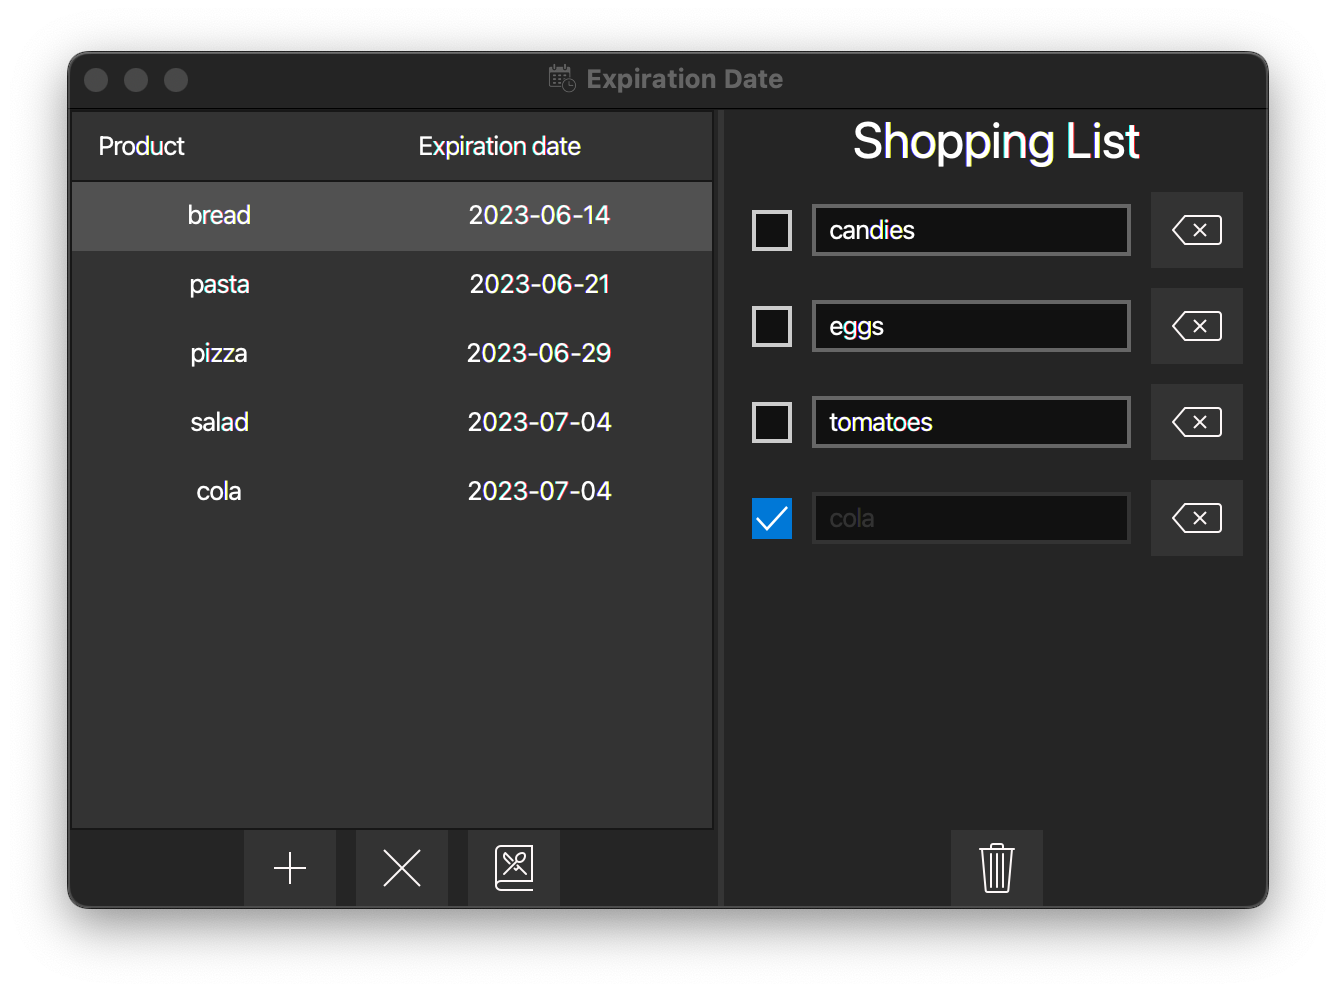
\includegraphics[width=\linewidth]{images/main-view.png}
    \caption{Finestra per la gestione di dispensa e lista della spesa.}
    \label{fig:mainview}
\end{figure}

La schermata per la gestione della dispensa e della lista della spesa si divide in due parti:

\begin{itemize}
  \item la parte di sinistra permette di aggiungere prodotti alla dispensa, eliminare prodotti dalla dispensa, modificare i dati di un prodotto o passare alla schermata delle ricette
  \begin{itemize}
    \item nel caso si desideri modificare i dati di un prodotto comparirà una schermata apposita per la modifica

    \begin{figure}[H]
        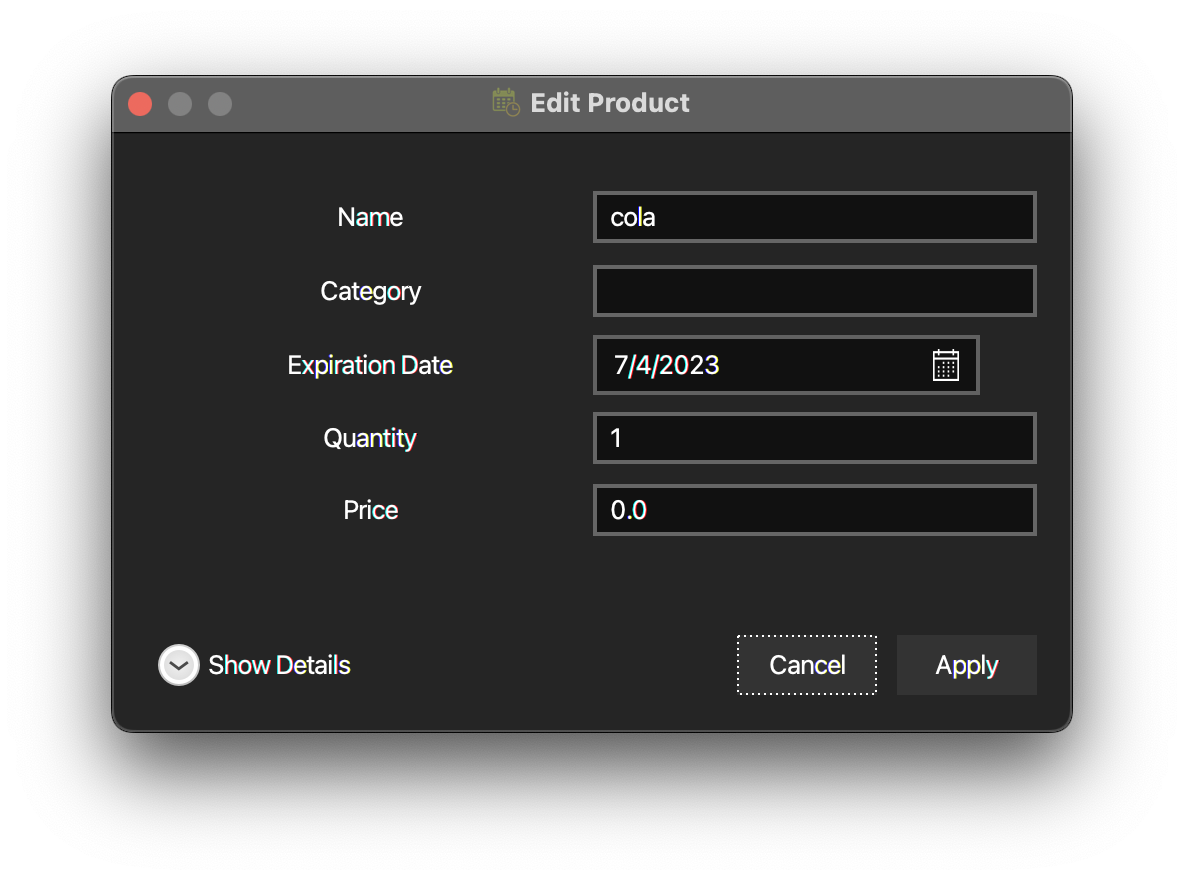
\includegraphics[width=\linewidth]{images/edit-product.png}
        \caption{Finestra per la modifica dei dati del prodotto.}
        \label{fig:editproduct}
    \end{figure}

  \end{itemize}
  \item la parte di destra permette di aggiungere prodotti alla lista della spesa, eliminare prodotti dalla lista della spesa, contrassegnare un prodotto della lista della spesa come "acquistato" (e aggiungerlo in automatico alla dispensa) e rimuovere tutti i prodotti contrassegnati come acquistati
\end{itemize}

\newpage

La schermata per la gestione delle ricette permette di navigare tra le ricette con le apposite frecce, aggiungere una ricetta, rimuovere una ricetta, modificare i dati di una ricetta, importare ed esportare liste di ricette.

\begin{figure}[H]
    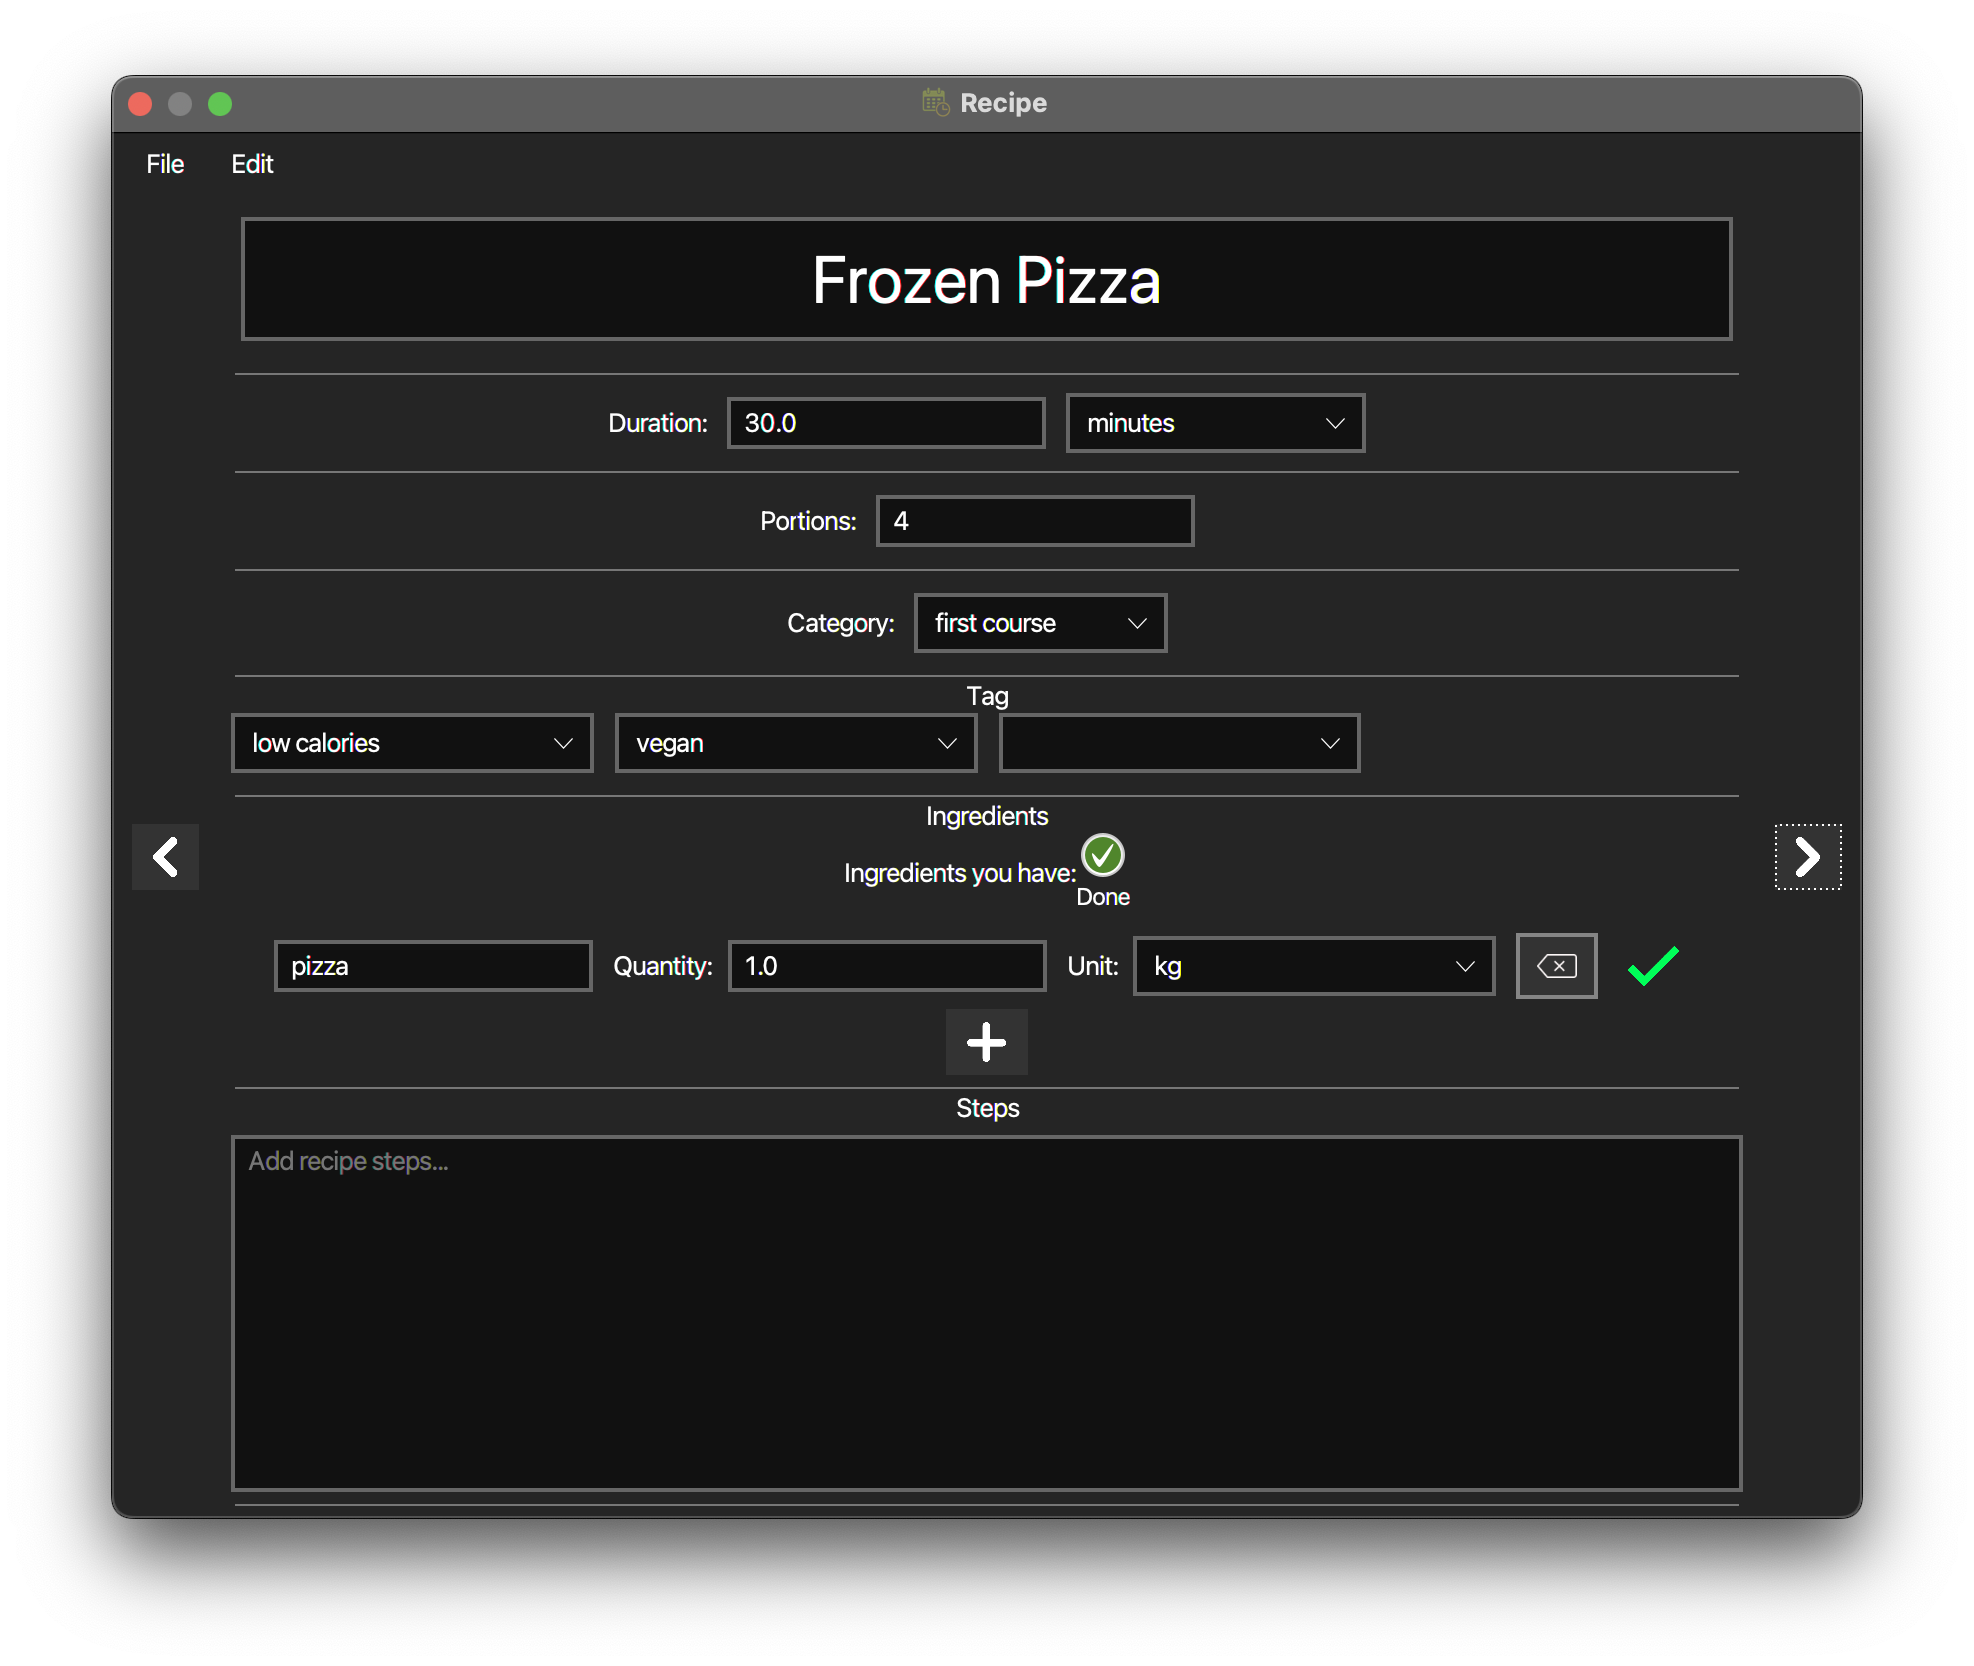
\includegraphics[width=\linewidth]{images/recipe-view.png}
    \caption{Finestra per la gestione delle ricette.}
    \label{fig:recipeview}
\end{figure}
